\chapter{Aufbau}
\textit{Ein Blick genügt: Der Aufbau von PUMA ist durchschaubar. Durch ausprobieren lernt man ihn am Besten kennen.}
\begin{figure}[h!]
 \centering
 \fbox{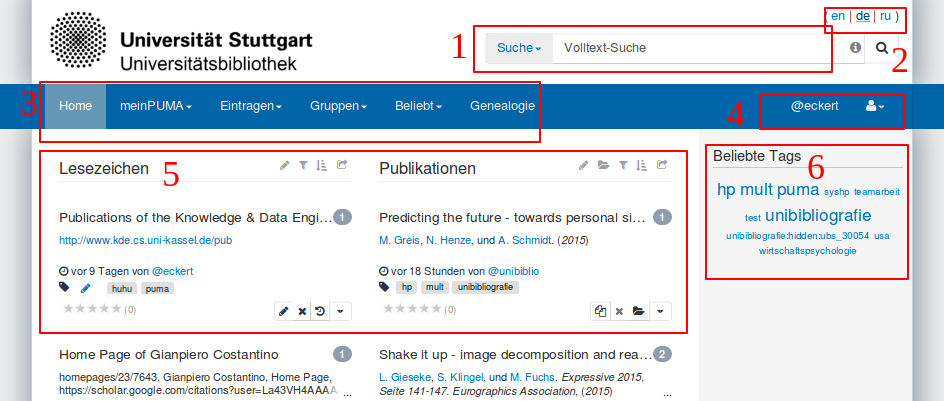
\includegraphics[width=12cm]{Bilder/Kapitel4/Puma_Hauptmenue}}
 \caption{Hauptmenü}
 \label{figure003}
\end{figure} 
\section{Suchleiste}
Die Suche\index{Suche} bei PUMA bietet viele Möglichkeiten den Datensatz nach unterschiedlichen Informationen zu durchsuchen. Durch das Klicken auf den kleinen Pfeil neben \enquote{Suche}\index{Suche} erscheint ein Dropdown-Menü. Der zu durchsuchende Datensatz wird durch anklicken ausgewählt. Anschließend wird der Suchbegriff in das weiße Feld daneben eingegeben. Durch das Klicken auf \enquote{Suche} oder \enquote{Enter} gibt PUMA in wenigen Sekunden die entsprechende Ergebnisse aus.

\begin{figure}[h!]
 \centering
 \fbox{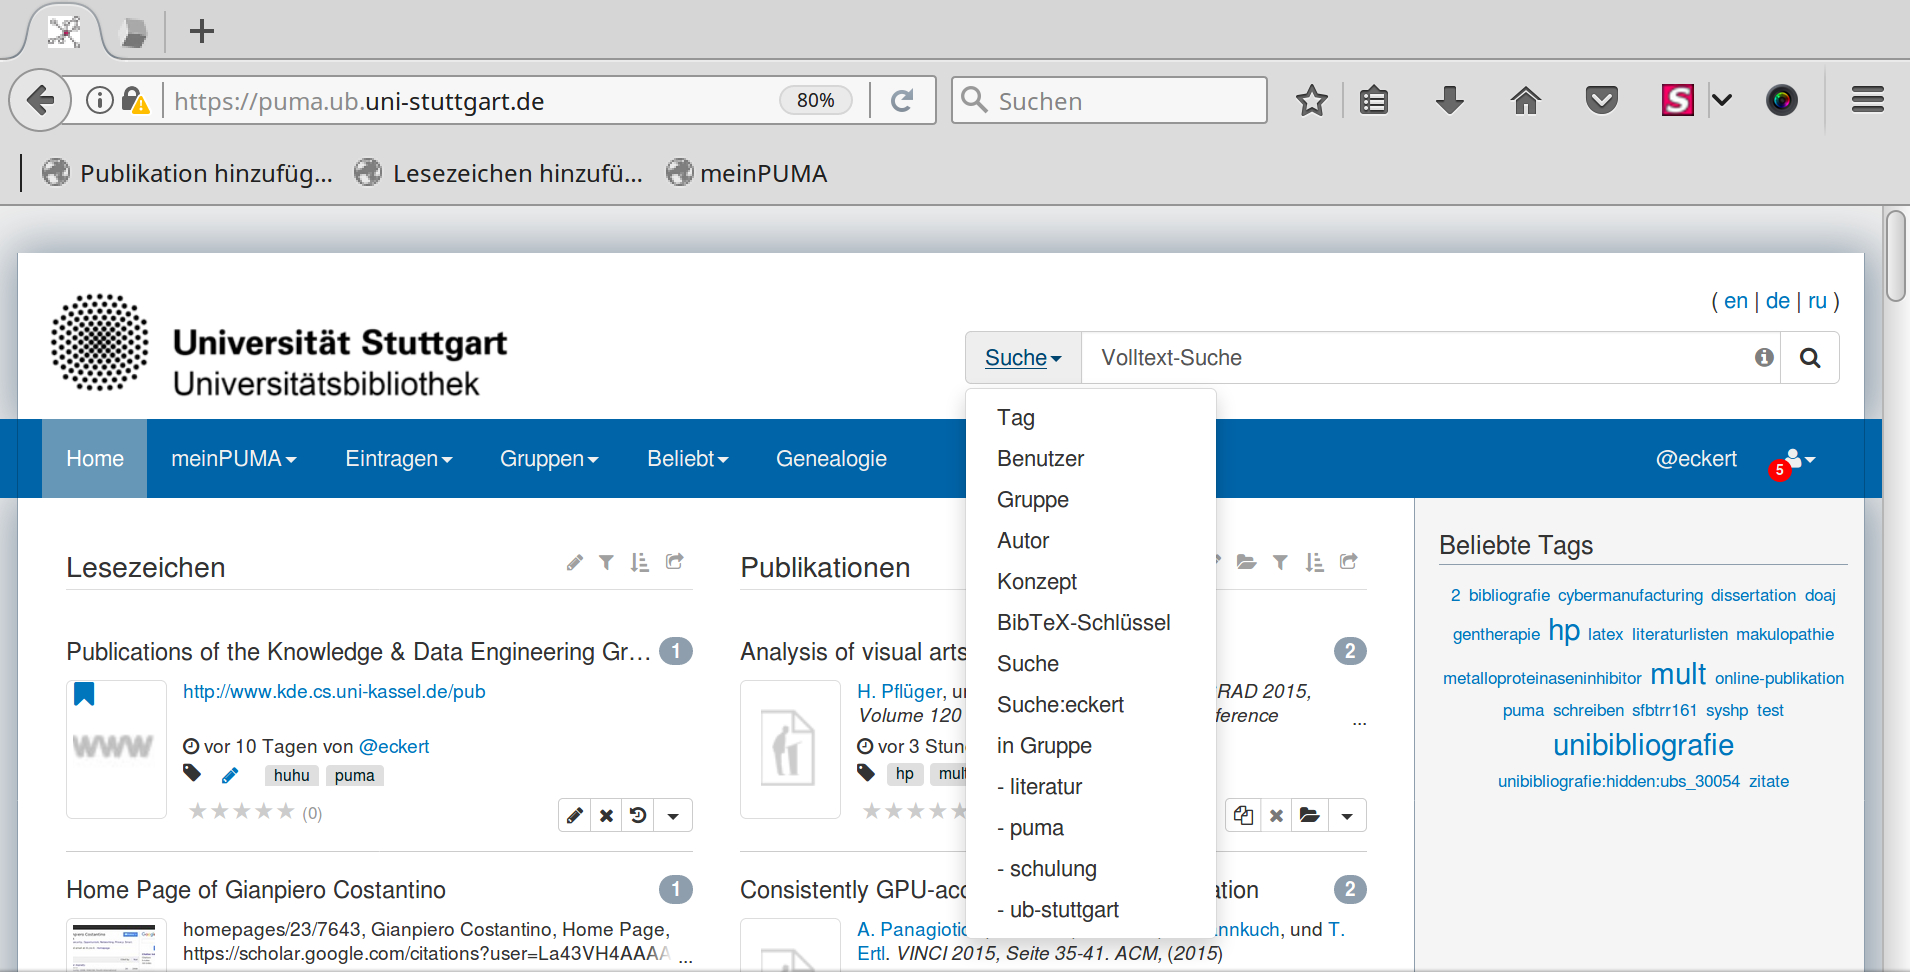
\includegraphics[width=10cm]{Bilder/Kapitel4/Suchleiste}}
 \caption{Suchleiste}
 \label{figure004}
\end{figure}  

\section{Spracheinstellung}
Hier haben Sie die Möglichkeit zwischen den drei verfügbaren Sprachen\index{Sprachen} in PUMA zu wechseln. Es gibt die Möglichkeiten zwischen Englisch (en), Deutsch (de) und Russisch (ru) zu wählen.
%\begin{wrapfigure}{l}{5cm}
\begin{mdframed}[style=tipp] \texttt{Um die Sprache für die Seite festzulegen, sodass diese bei jedem neuen Besuch bei PUMA gleich ist, müssen Sie dies in den Einstellungen festlegen. Dorthin gelangen Sie über das Personensymbol rechts im Hauptmenü. Klicken Sie auf den Reiter \enquote{Einstellungen} und die Seite mit den Einstellungen öffnet sich. Anschließend klicken Sie auf die Rubrik \enquote{Einstellungen}. Auf der erscheinenden Seite können Sie nun die gewünschte Sprache festlegen und müssen anschließend auf \enquote{Layout speichern} die Änderung bestätigen.}
\end{mdframed}
%\end{wrapfigure}
  

\section{Linkes Hauptmenü} 
Das Hauptmenü stellt die wichtigsten Funktionen von PUMA bereit. Es ist zu beachten, dass sich einige Einstellungen unterscheiden, da es bei PUMA die Unterscheidung zwischen einfachen Funktionen\index{Funktionen!Einfache} und erweiterten Funktionen\index{Funktionen!Erweiterte} gibt. Dies betrifft vor allem den unten genannten Punkt \enquote{Mein PUMA}. 
\subsection{Home\index{Home}}
Damit gelangen Sie zur Startseite und erhalten einen Überblick über Publikationen und Lesezeichen, die vor kurzer Zeit eingetragen wurden. In jeder der beiden Spalten können Sie separate Einstellungen für die Publikationen oder Lesezeichen vornehmen. Mit dem schwarzen Stift können alle eigenen Einträge in der Liste bearbeitet werden, der Trichter ermöglicht es ihnen, die angezeigten Einträge zu filtern, mit dem Pfeil nach unten können Sie die Reihenfolge und Sortierung der angezeigten Einträge ändern und mit dem Exportzeichen können Sie die Exportmöglichkeiten für die angezeigten Einträge festlegen.
\subsection{Mein PUMA\index{Mein PUMA}}
Es ist zu beachten, dass sich einige Einstellungen unterscheiden, da es bei PUMA die Unterscheidung zwischen einfachen Funktionen\index{Funktionen} und erweiterten Funktionen gibt. Durch das Freischalten der erweiterten Funktionen kommen weitere Funktionen hinzu.
\begin{enumerate}
    \item Einfache Funktion\index{Funktionen!Einfache}:
    \begin{itemize}
        \item meine Einträge\index{Einträge}: Hier gelangen Sie zu dem eigenen Publikations- und Lesezeichenverzeichnis, das Sie sich angelegt haben.
        \item diskutierte Einträge\index{Einträge!diskutierte}: Hier finden Sie alle Publikationen und Lesezeichen, die Sie selber bewertet haben. Ebenso werden Kommentare und Rezessionen von anderen Nutzern zu Ihren Publikationen hier angezeigt.
        \item verfolgte Einträge\index{Einträge!verfolgen}: Hier werden Ihnen alle Publikationen und Lesezeichen der Nutzer angezeigt, denen Sie folgen.
        \item Einträge von Freunden\index{Einträge!von Freunden}: Es werden Ihnen alle Einträge Ihrer Freunde angezeigt.
    \end{itemize}
    \item Erweiterte Funktionen\index{Funktionen!Erweiterte}:
    \begin{itemize}
        \item private Einträge\index{Einträge!privat}: Damit gelangen Sie zu Ihren Einträgen, die nur für Sie sichtbar sind. 
        \item Einträge für Freunde\index{Einträge!Freunde}: Zeigt die Einträge, die nur Sie selber und Ihre Freunde sehen können.
        \item Dokumente\index{Dokumente}: Wenn Sie Ihren Einträgen Dokumente (z.B. eine PDF-Datei) angehängt haben, können Sie hier eine Übersicht über die angehängten Dokumente sehen.
        \item Duplikate\index{Duplikate}: Zeigt Ihnen die Einträge, die wahrscheinlich Duplikate sind. So können Sie ihre Literaturliste ganz einfach bereinigen. 
        \item Konzepte\index{Konzepte}: Konzepte ermöglichen es Ihnen mehreren Schlagwörtern zu gruppieren. 
        \item Lebenslauf\index{Konzepte}: Hier können Sie Ihre persönlichen Daten hinterlegen, welche für andere Nutzer in PUMA sichtbar sind.
        \item Publikationen durchstöbern: Mit dieser Funktion können Sie Ihre eigenen Lesezeichen/~Publikationen durchstöbern. Sie erhalten so einen schnellen Überblick über den eigenen Literaturbestand. 
        \item BibTex\index{BibTex} exportieren: Exportiert Ihre Daten in das BibTex-Format.
    \end{itemize}
\end{enumerate}
\subsection{Eintragen}
\begin{enumerate}
    \item Lesezeichen eintragen\index{Lesezeichen!eintragen}: Fügen Sie ein neues Lesezeichen Ihrer Sammlung hinzu.  
    \item Publikation eintragen\index{Publikationen!eintragen}: Fügen Sie ein neue Publikation Ihrer Sammlung hinzu. 
    \item Lesezeichen importieren\index{Lesezeichen!Import}: Importieren Sie Lesezeichen aus Ihrem Browser oder Ihren Delicious Daten.
    \item Publikationen importieren\index{Publikationen!Import}: Importieren Sie eine bestehende BibTeX- oder EndNote-Datei in PUMA.
\end{enumerate}


\subsection{Gruppen}
Zeigt Ihnen die Funktionen zu Gruppen\index{Gruppen} an sowie die Gruppen in denen Sie Mitglied sind.
\begin{enumerate}
    \item Alle Gruppen: Verschafft Ihnen einen Überblick über alle existierenden Gruppen bei PUMA.
    \item Eine neue Gruppe erstellen: Bietet Ihnen die Möglichkeit eine eigene Gruppe zu erstellen.
\end{enumerate}
\subsection{Beliebt\index{Beliebt}}
Ermöglicht Ihnen, die derzeitig beliebtesten Einträge bei PUMA zu durchforsten.
\begin{enumerate}
    \item Einträge: Zeigt die beliebtesten Einträge an.
    \item Tags: Zeigt die beliebtesten Tags in einer Schlagwortwolke an. Je größer ein Tag ist, desto beliebter ist er.
    \item Autor: Zeigt die beliebtesten Autoren an.
    \item Konzepte: Zeigt die beliebtesten Konzepte und deren Zuordnungen an. 
    \item Diskussionen: Zeigt Lesezeichen und Publikationen an, über welche viel diskutiert wurde. 
\end{enumerate}
\subsection{Genealogie}
Die PUMA Genealogie erstellt nutzerbasiert einen Stammbaum der Forschung an deutschen Universitäten. Ausgangspunkt ist der Dissertationskatalog der Deutschen Nationalbibliothek. Nutzerbasiert werden Beziehungen zwischen den an der Dissertation beteiligten Personen (Autor\_in, Betreuer\_in etc.) ergänzt.

\section{Rechtes Hauptmenü}
\subsection{@username\index{@username}}
Über diesen Button gelangen Sie zu Ihrer Publikations- und Lesezeichensammlung. 
\subsection{Das Personensymbol}
\begin{enumerate}
    \item Eingang\index{Eingang}: Dies ist Ihr Lesenzeichen-/~Publikations-Posteingang. Freunde/Gruppen können Ihnen Publikationen und Lesezeichen zuschicken, diese Eingänge landen dann hier.
    \item Ablage\index{Ablage}: In der Ablage können Sie aktuelle Literaturlisten zusammenstellen. 
    \item Freunde\index{Freunde}: Hier erhalten Sie einen Überblick über Ihre Freunde. 
    \item Tags bearbeiten\index{Tags!bearbeiten}: Hier können Sie Tags und Konzepte überarbeiten, beispielsweise alte Tags durch neue ersetzten. 
    \item Einstellungen\index{Einstellungen}: Zeigt Ihre persönlichen Benutzereinstellungen an. Sie können hier Ihr Profil, die allgemeinen Einstellungen, Ihren Lebenslauf sowie Einstellungen zu Gruppen ändern.
    \item Weblog\index{Weblog}: Leitet Sie zu dem Weblog\footnote{\url{http://blog.ub.uni-stuttgart.de/category/puma/}} von PUMA weiter.
    \item Hilfe\index{Hilfe}: Damit gelangen Sie zur Online-Hilfe.
    \item Abmelden\index{Abmelden}: Wenn Sie PUMA verlassen wollen, melden Sie sich hier ab. 
\end{enumerate}

\textbf{Der PUMA-Aufbau im Überblick}
%\small

\tabulinesep=1.5mm
\begin{longtabu}{|X[l]|X[l]|X[l]|X[l]|}\hline
\rowfont\bfseries
Hauptmenü & Untermenü & Reiter & Rubrik\\  \hline
\endfirsthead
\hline
%\multicolumn{4}{@{}l}{\small\dots\emph{Fortsetzung}}\\ \hline
\rowfont\bfseries
Hauptmenü & Untermenü & Reiter & Rubrik\\  \hline
\endhead
\hline
%\multicolumn{4}{@{}l}{\small\dots\emph{Fortsetzung nächste Seite} \ldots}\\ \hline
\endfoot
%\hline
\endlastfoot
Eintragen&Lesezeichen eintragen &- &-\\ \cline{2-4}
&Publikation eintragen &Per Hand& Tragen Sie Ihre Publikation hier ein\\\cline{3-4}
&&BibTex/EndNote-Schnipsel& Tragen Sie hier Ihre BibTex- oder EndNote-Schnipsel ein\\ \cline{4-4}
&&& Einstellungen\\ \cline{3-4}
&&Datei hochladen& Laden Sie ihre BibTex- oder EndNote-Datei hier hoch\\ \cline{4-4}
&&&Einstellungen\\ \cline{3-4}
&&ISBN/DOI& ISBN\\ \cline{4-4}
&&& ISSN \\ \cline{4-4}
&&&DOI\\ \cline{3-4}
&&Code scannen&-\\ \cline{2-4}
&Lesezeichen importieren&- &Importieren Sie Ihre Lesezeichen aus Ihrem Browser\\ \cline{4-4}
&& & Importieren Sie Ihre Delicious Daten\\ \cline{2-4} 
&Publikationen importieren &-&-\\ \hline
Gruppen&Alle Gruppen& Gruppen von A-Z &-\\ \cline{2-4}
&Gruppen, in denen der Nutzer Mitglied ist& Einträge &-\\\cline{3-4}
&&Interessant für &- \\ \cline{3-4}
&&Sichtbar&-\\ \cline{3-4}
&&Dokumente&-\\ \cline{3-4}
&&diskutierte Einträge&-\\ \cline{3-4}
&&Einstellungen&Gruppeneinstellungen und Mitgliederliste\\ \cline{2-4}
&Eine neue Gruppe erstellen&-&-\\ \hline
Personensymbol&Eingang&-&-\\ \cline{2-4}
&Ablage&-&-\\ \cline{2-4}
&Freunde&Ihre Freunde&- \\ \cline{3-4}
&&Sie sind ein Freund von&- \\ \cline{2-4}
&Tags bearbeiten&-&Umbenennen/ Ersetzen von Tags\\ \cline{4-4}
&&&Subtags zu Konzepten hinzufügen\\ \cline{4-4}
&&&Subtags von Konzept löschen\\ \cline{2-4}
&Einstellungen&Mein Profil&Allgemeine Informationen\\ \cline{4-4}
&&&Kontakt\\ \cline{4-4}
&&&Über mich\\ \cline{4-4}
&&&Ein Bild für meinen Lebenslauf\\\cline{3-4}
&&Einstellungen&Layouts Ihrer Tagbox und Ihrer Eintragsbilder\\\cline{4-4}
&&&API\\\cline{4-4}
&&&Logging und Löschen\\\cline{4-4}
&&&Passwort ändern\\\cline{4-4}
&&&Mein Konto löschen\\\cline{3-4}
&&JabRef Layout-Datei&-\\\cline{3-4}
&&Lebenslauf& Lebenslauf editieren\\\cline{4-4}
&&&Layout editieren\\ \cline{4-4}
&&&Vorschau wird erzeugt\\\cline{3-4}
&&OAuth-Consumers&- \\\cline{3-4}
&&Gruppen&Eine neue Gruppe erstellen\\\cline{4-4}
&&&Gruppen\\\cline{2-4}
&Einstellungen&Synchronisation&-\\\cline{2-4}
&Weblog&-&-\\\cline{2-4}
&Hilfe&-&-\\\cline{2-4}
&Abmelden&-&-\\\hline
\caption{Der PUMA-Aufbau im Überblick}
\end{longtabu}

%\normalsize

\section{Inhaltsbereich}
Hier sehen Sie die aktuellsten Lesezeichen und Publikationen von Ihnen und anderen Nutzern. 
\section{Beliebte Tags}
Zeigt Ihnen die beliebtesten Tags\index{Tags} an. Sie können zwischen der Wolken- oder Listen-Ansicht wählen.